\documentclass[9pt]{beamer}
\usetheme{cmepda}

\usepackage[utf8]{inputenc}
\usepackage[T1]{fontenc}


\title{numpy and scipy (1/2)}
\subtitle{Computing Methods for Experimental Physics and Data Analysis}
\date{Compiled on \today}
\author{L. Baldini}
\institute[UNIPI and INFN]{Universit\`a and INFN--Pisa}
\email{luca.baldini@pi.infn.it}


\begin{document}


\titleframe

\begin{frame}
  \frametitle{Introduction}
  \begin{itemize}
  \item Python is notorious for coming \emph{with batteries included}\ldots
  \item \ldots but as a data scientist numpy and and scipy will be your
    best friends!
  \item Among (many) other things, numpy offers:
    \begin{itemize}
    \item a powerful n-dimensional array object
    \item mathematical functions that interoperate natively with arrays
    \end{itemize}
  \item And scipy provides:
    \begin{itemize}
    \item integration
    \item optimization (a.k.a. fitting)
    \item interpolation
    \item signal processing
    \end{itemize}
  \end{itemize}
\end{frame}


\begin{frame}
  \frametitle{numpy arrays}
  \begin{Verbatim}[label=\makebox{\url{https://github.com/lucabaldini/cmepda/tree/master/slides/latex/snippets/numpy\_arrays.py}},commandchars=\\\{\}]
\PY{k+kn}{import} \PY{n+nn}{numpy} \PY{k+kn}{as} \PY{n+nn}{np}

\PY{c+c1}{\PYZsh{} Initialization from a list}
\PY{n}{a1} \PY{o}{=} \PY{n}{np}\PY{o}{.}\PY{n}{array}\PY{p}{(}\PY{p}{[}\PY{l+m+mf}{1.}\PY{p}{,} \PY{l+m+mf}{2.}\PY{p}{,} \PY{l+m+mi}{3}\PY{p}{]}\PY{p}{)}
\PY{k}{print}\PY{p}{(}\PY{n}{a1}\PY{p}{)}

\PY{c+c1}{\PYZsh{} Zeros, ones, and fixed values}
\PY{n}{a2} \PY{o}{=} \PY{n}{np}\PY{o}{.}\PY{n}{zeros}\PY{p}{(}\PY{l+m+mi}{10}\PY{p}{)}
\PY{n}{a3} \PY{o}{=} \PY{n}{np}\PY{o}{.}\PY{n}{ones}\PY{p}{(}\PY{p}{(}\PY{l+m+mi}{2}\PY{p}{,} \PY{l+m+mi}{2}\PY{p}{)}\PY{p}{)}
\PY{n}{a4} \PY{o}{=} \PY{n}{np}\PY{o}{.}\PY{n}{full}\PY{p}{(}\PY{l+m+mi}{7}\PY{p}{,} \PY{l+m+mf}{3.}\PY{p}{)}
\PY{k}{print}\PY{p}{(}\PY{n}{a2}\PY{p}{)}
\PY{k}{print}\PY{p}{(}\PY{n}{a3}\PY{p}{)}
\PY{k}{print}\PY{p}{(}\PY{n}{a4}\PY{p}{)}

\PY{c+c1}{\PYZsh{} Grids}
\PY{n}{a5} \PY{o}{=} \PY{n}{np}\PY{o}{.}\PY{n}{linspace}\PY{p}{(}\PY{l+m+mf}{0.}\PY{p}{,} \PY{l+m+mf}{10.}\PY{p}{,} \PY{l+m+mi}{11}\PY{p}{)}
\PY{n}{a6} \PY{o}{=} \PY{n}{np}\PY{o}{.}\PY{n}{logspace}\PY{p}{(}\PY{l+m+mf}{0.}\PY{p}{,} \PY{l+m+mf}{1.}\PY{p}{,} \PY{l+m+mi}{11}\PY{p}{)}
\PY{k}{print}\PY{p}{(}\PY{n}{a5}\PY{p}{)}
\PY{k}{print}\PY{p}{(}\PY{n}{a6}\PY{p}{)}

[Output]
[1. 2. 3.]
[0. 0. 0. 0. 0. 0. 0. 0. 0. 0.]
[[1. 1.]
 [1. 1.]]
[3. 3. 3. 3. 3. 3. 3.]
[ 0.  1.  2.  3.  4.  5.  6.  7.  8.  9. 10.]
[ 1.          1.25892541  1.58489319  1.99526231  2.51188643  3.16227766
  3.98107171  5.01187234  6.30957344  7.94328235 10.        ]
\end{Verbatim}
\end{frame}


\begin{frame}
  \frametitle{numpy arrays vs. Python lists}
  \begin{Verbatim}[label=\makebox{\url{https://bitbucket.org/lbaldini/programming/src/tip/snippets/numpy\_arrays\_vs\_lists.py}},commandchars=\\\{\}]
\PY{k+kn}{import} \PY{n+nn}{numpy} \PY{k+kn}{as} \PY{n+nn}{np}

\PY{c+c1}{\PYZsh{} arrays and lists seem similar...}
\PY{n}{l} \PY{o}{=} \PY{p}{[}\PY{l+m+mf}{1.}\PY{p}{,} \PY{l+m+mf}{2.}\PY{p}{,} \PY{l+m+mf}{3.}\PY{p}{]}
\PY{n}{a} \PY{o}{=} \PY{n}{np}\PY{o}{.}\PY{n}{array}\PY{p}{(}\PY{n}{l}\PY{p}{)}
\PY{k}{print}\PY{p}{(}\PY{n}{l}\PY{p}{)}
\PY{k}{print}\PY{p}{(}\PY{n}{a}\PY{p}{)}

\PY{c+c1}{\PYZsh{} ...but they support basic arithmetic in a different fashion}
\PY{k}{print}\PY{p}{(}\PY{n}{l} \PY{o}{+} \PY{n}{l}\PY{p}{)}
\PY{k}{print}\PY{p}{(}\PY{n}{a} \PY{o}{+} \PY{n}{a}\PY{p}{)}

[Output]
[1.0, 2.0, 3.0]
[1. 2. 3.]
[1.0, 2.0, 3.0, 1.0, 2.0, 3.0]
[2. 4. 6.]
\end{Verbatim}
  
  \begin{itemize}
  \item arrays and lists are fundamentally different objects
    \begin{itemize}
    \item different footprint in memory, operate at different speed
    \item arrays are homogeneous, lists don't need to
    \item arrays offer a much more powerful indexing/slicing
    \item arrays interoperate with numpy mathematical functions
    \end{itemize}
  \end{itemize}
\end{frame}


\begin{frame}
  \frametitle{Broadcasting}
  \begin{Verbatim}[label=\makebox{\url{https://github.com/lucabaldini/cmepda/tree/master/slides/latex/snippets/numpy\_arrays\_broadcasting.py}},commandchars=\\\{\}]
\PY{k+kn}{import} \PY{n+nn}{numpy} \PY{k+kn}{as} \PY{n+nn}{np}

\PY{n}{a1} \PY{o}{=} \PY{n}{np}\PY{o}{.}\PY{n}{array}\PY{p}{(}\PY{p}{[}\PY{l+m+mf}{1.}\PY{p}{,} \PY{l+m+mf}{2.}\PY{p}{]}\PY{p}{)}
\PY{n}{a2} \PY{o}{=} \PY{n}{np}\PY{o}{.}\PY{n}{array}\PY{p}{(}\PY{p}{[}\PY{p}{[}\PY{l+m+mf}{1.}\PY{p}{,} \PY{l+m+mf}{2.}\PY{p}{]}\PY{p}{,} \PY{p}{[}\PY{l+m+mf}{3.}\PY{p}{,} \PY{l+m+mf}{4.}\PY{p}{]}\PY{p}{]}\PY{p}{)}
\PY{n}{c} \PY{o}{=} \PY{n}{np}\PY{o}{.}\PY{n}{pi}

\PY{k}{print}\PY{p}{(}\PY{n}{a1}\PY{p}{)}
\PY{k}{print}\PY{p}{(}\PY{n}{a2}\PY{p}{)}
\PY{k}{print}\PY{p}{(}\PY{n}{c}\PY{p}{)}
\PY{k}{print}\PY{p}{(}\PY{n}{a1} \PY{o}{*} \PY{n}{a1}\PY{p}{)}
\PY{k}{print}\PY{p}{(}\PY{n}{a1} \PY{o}{*} \PY{n}{c}\PY{p}{)}
\PY{k}{print}\PY{p}{(}\PY{n}{a1} \PY{o}{*} \PY{n}{a2}\PY{p}{)}

[Output]
[1. 2.]
[[1. 2.]
 [3. 4.]]
3.141592653589793
[1. 4.]
[3.14159265 6.28318531]
[[1. 4.]
 [3. 8.]]
\end{Verbatim}
  
  \begin{itemize}
  \item Under certain conditions, numpy can make operations on arrays of
    different shape
  \item This is extremely useful when vectorizing problems 
  \end{itemize}
\end{frame}


\begin{frame}
  \frametitle{Mathematical functions in numpy}
  \begin{Verbatim}[label=\makebox{\url{https://github.com/lucabaldini/cmepda/tree/master/slides/latex/snippets/numpy\_functions.py}},commandchars=\\\{\}]
\PY{k+kn}{import} \PY{n+nn}{numpy} \PY{k+kn}{as} \PY{n+nn}{np}
\PY{k+kn}{import} \PY{n+nn}{math}

\PY{n}{a} \PY{o}{=} \PY{n}{np}\PY{o}{.}\PY{n}{array}\PY{p}{(}\PY{p}{[}\PY{l+m+mf}{0.1}\PY{p}{,} \PY{l+m+mf}{1.}\PY{p}{,} \PY{l+m+mf}{10.}\PY{p}{]}\PY{p}{)}

\PY{k}{print}\PY{p}{(}\PY{n}{np}\PY{o}{.}\PY{n}{log10}\PY{p}{(}\PY{n}{a}\PY{p}{)}\PY{p}{)}
\PY{k}{print}\PY{p}{(}\PY{n}{np}\PY{o}{.}\PY{n}{exp}\PY{p}{(}\PY{n}{a}\PY{p}{)}\PY{p}{)}
\PY{k}{print}\PY{p}{(}\PY{n}{np}\PY{o}{.}\PY{n}{sin}\PY{p}{(}\PY{n}{a}\PY{p}{)}\PY{p}{)}

\PY{k}{print}\PY{p}{(}\PY{n}{np}\PY{o}{.}\PY{n}{log10}\PY{p}{(}\PY{l+m+mf}{0.1}\PY{p}{)}\PY{p}{)}

\PY{k}{print}\PY{p}{(}\PY{n}{math}\PY{o}{.}\PY{n}{log10}\PY{p}{(}\PY{n}{a}\PY{p}{)}\PY{p}{)}

[Output]
[-1.  0.  1.]
[1.10517092e+00 2.71828183e+00 2.20264658e+04]
[ 0.09983342  0.84147098 -0.54402111]
-1.0
Traceback (most recent call last):
  File "snippets/numpy_functions.py", line 12, in <module>
    print(math.log10(a))
TypeError: only size-1 arrays can be converted to Python scalars
\end{Verbatim}
  
  \begin{itemize}
  \item numpy mathematical functions interoperate natively with arrays
    \begin{itemize}
    \item (and work on plain old numbers, too)
    \end{itemize}
  \end{itemize}
\end{frame}


\begin{frame}
  \frametitle{Arrays and masks}
  \begin{Verbatim}[label=\makebox{\url{https://bitbucket.org/lbaldini/programming/src/tip/snippets/numpy\_masks.py}},commandchars=\\\{\}]
\PY{k+kn}{import} \PY{n+nn}{numpy} \PY{k+kn}{as} \PY{n+nn}{np}

\PY{n}{a} \PY{o}{=} \PY{n}{np}\PY{o}{.}\PY{n}{linspace}\PY{p}{(}\PY{l+m+mf}{0.}\PY{p}{,} \PY{l+m+mf}{10.}\PY{p}{,} \PY{l+m+mi}{11}\PY{p}{)}
\PY{n}{mask1} \PY{o}{=} \PY{n}{a} \PY{o}{\PYZgt{}}\PY{o}{=} \PY{l+m+mf}{2.5}
\PY{n}{mask2} \PY{o}{=} \PY{n}{a} \PY{o}{\PYZlt{}} \PY{l+m+mf}{8.5}

\PY{k}{print}\PY{p}{(}\PY{n}{a}\PY{p}{)}
\PY{k}{print}\PY{p}{(}\PY{n}{mask1}\PY{p}{)}
\PY{k}{print}\PY{p}{(}\PY{n}{mask2}\PY{p}{)}
\PY{k}{print}\PY{p}{(}\PY{n}{a}\PY{p}{[}\PY{n}{mask1}\PY{p}{]}\PY{p}{)}
\PY{k}{print}\PY{p}{(}\PY{n}{a}\PY{p}{[}\PY{n}{mask2}\PY{p}{]}\PY{p}{)}
\PY{k}{print}\PY{p}{(}\PY{n}{a}\PY{p}{[}\PY{n}{np}\PY{o}{.}\PY{n}{logical\PYZus{}and}\PY{p}{(}\PY{n}{mask1}\PY{p}{,} \PY{n}{mask2}\PY{p}{)}\PY{p}{]}\PY{p}{)}

[Output]
[ 0.  1.  2.  3.  4.  5.  6.  7.  8.  9. 10.]
[False False False  True  True  True  True  True  True  True  True]
[ True  True  True  True  True  True  True  True  True False False]
[ 3.  4.  5.  6.  7.  8.  9. 10.]
[0. 1. 2. 3. 4. 5. 6. 7. 8.]
[3. 4. 5. 6. 7. 8.]
\end{Verbatim}
  
  \begin{itemize}
  \item Masks are a powerful tool in numpy
  \item They can replace conditional expressions in a for loop in
    vectorization context (more on this later)
  \end{itemize}
\end{frame}


\begin{frame}[fragile]
  \frametitle{Digression: pseudo-random number generators}

  \begin{Verbatim}
    import random
    x = random.random()
  \end{Verbatim}

  \medskip
  
  \begin{itemize}
  \item Every programming language comes with a Pseudo Random Number
    Generator (PRNG)
    \begin{itemize}
    \item Python is no exception:
      \url{https://docs.python.org/3/library/random.html}
    \item Mersenne-Twister, 53-bit precision, period of $2^{19937} - 1$. 
    \end{itemize}
  \item PRNGs are an interesting (and fun) subject by themselves:
    \begin{itemize}
    \item Donald E. Knuth, \emph{The Art of Computer Programming, Volume 2: Seminumerical Algorithms}, 3rd Edition 
    \item M. Matsumoto and T. Nishimura, \emph{Mersenne Twister: A 623-dimensionally equidistributed uniform pseudorandom number generator}, ACM Transactions on Modeling and Computer Simulation Vol. 8, No. 1, January pp.3--30 1998.
    \end{itemize}
  \item A PRNG produces random floats uniformly in $[0.0,~1.0)$.
  \end{itemize}
\end{frame}


\begin{frame}
  \frametitle{Vectorization}
  \framesubtitle{a.k.a. avoid explicit for loops in Python whenever you can}
  \begin{Verbatim}[label=\makebox{\url{https://github.com/lucabaldini/cmepda/tree/master/slides/latex/snippets/vectorization.py}},commandchars=\\\{\}]
\PY{k+kn}{import} \PY{n+nn}{random}
\PY{k+kn}{import} \PY{n+nn}{time}
\PY{k+kn}{import} \PY{n+nn}{numpy} \PY{k+kn}{as} \PY{n+nn}{np}

\PY{c+c1}{\PYZsh{} How many random numbers (uniformly distributed between 0 and 1) do you}
\PY{c+c1}{\PYZsh{} want to throw?}
\PY{n}{n} \PY{o}{=} \PY{l+m+mi}{1000000}

\PY{c+c1}{\PYZsh{} The slow way: explicit for loop in Python.}
\PY{n}{t0} \PY{o}{=} \PY{n}{time}\PY{o}{.}\PY{n}{time}\PY{p}{(}\PY{p}{)}
\PY{n}{x} \PY{o}{=} \PY{p}{[}\PY{p}{]}
\PY{k}{for} \PY{n}{i} \PY{o+ow}{in} \PY{n+nb}{range}\PY{p}{(}\PY{n}{n}\PY{p}{)}\PY{p}{:}
    \PY{n}{x}\PY{o}{.}\PY{n}{append}\PY{p}{(}\PY{n}{random}\PY{o}{.}\PY{n}{random}\PY{p}{(}\PY{p}{)}\PY{p}{)}
\PY{n}{dt} \PY{o}{=} \PY{n}{time}\PY{o}{.}\PY{n}{time}\PY{p}{(}\PY{p}{)} \PY{o}{\PYZhy{}} \PY{n}{t0}
\PY{k}{print}\PY{p}{(}\PY{l+s+s1}{\PYZsq{}}\PY{l+s+s1}{Elapsed time: }\PY{l+s+si}{\PYZpc{}.3f}\PY{l+s+s1}{ s}\PY{l+s+s1}{\PYZsq{}} \PY{o}{\PYZpc{}} \PY{n}{dt}\PY{p}{)}

\PY{c+c1}{\PYZsh{} The quick way: vectorizing in numpy}
\PY{n}{t0} \PY{o}{=} \PY{n}{time}\PY{o}{.}\PY{n}{time}\PY{p}{(}\PY{p}{)}
\PY{n}{x} \PY{o}{=} \PY{n}{np}\PY{o}{.}\PY{n}{random}\PY{o}{.}\PY{n}{random}\PY{p}{(}\PY{n}{size}\PY{o}{=}\PY{n}{n}\PY{p}{)}
\PY{n}{dt} \PY{o}{=} \PY{n}{time}\PY{o}{.}\PY{n}{time}\PY{p}{(}\PY{p}{)} \PY{o}{\PYZhy{}} \PY{n}{t0}
\PY{k}{print}\PY{p}{(}\PY{l+s+s1}{\PYZsq{}}\PY{l+s+s1}{Elapsed time: }\PY{l+s+si}{\PYZpc{}.3f}\PY{l+s+s1}{ s}\PY{l+s+s1}{\PYZsq{}} \PY{o}{\PYZpc{}} \PY{n}{dt}\PY{p}{)}

[Output]
Elapsed time: 0.137 s
Elapsed time: 0.015 s
\end{Verbatim}
\end{frame}


\begin{frame}
  \frametitle{How does vectorizaion work?}
  \begin{itemize}
  \item Python is know to be slooow
    \begin{itemize}
    \item This is the price you pay for being so beautiful and flexible
    \end{itemize}
  \item Does it matter? If depends\ldots
    \begin{itemize}
    \item If you are parsing a text file or fetching a web page probably not
    \item If you are performing a CPU-intensive processing on a TB of data
      probably yes
    \end{itemize}
  \item What's so magic in using numpy?
  \item numpy is written in C as a Python extension
    \begin{itemize}
    \item Routines are highly optimized to cruch numbers
    \item When you perform an array operation in Python you are actually
      executing optimized C code
    \end{itemize}
  \item \alert{Basic message: avoid for loops in pure Python when
    crunching numbers}
  \end{itemize}
\end{frame}


\begin{frame}
  \frametitle{How do I throw PRN with arbitrary pdf?}
  \framesubtitle{Hit or miss}
  \centering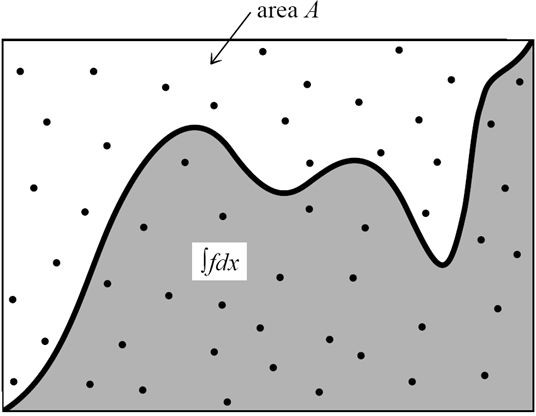
\includegraphics[width=0.5\textwidth]{hitmiss}

  \begin{itemize}
  \item Hit or miss, aka acceptance/rejection method:
    \begin{itemize}
    \item Enclose your pdf in a rectangle
    \item Throw a $x$ and a $y$
    \item Accept $x$ if $y \leq f(x)$
    \end{itemize}
  \item \alert{This is horrible---please don't use it!}
  \end{itemize}
\end{frame}


\begin{frame}
  \frametitle{How do I throw PRN with arbitrary pdf?}
  \framesubtitle{Inverse transform}
  \begin{itemize}
  \item Probability density function (pdf)
    $$
    p(x) \quad (\ge 0)
    $$
  \item Cumulative function (cf)
    $$
    F(x) = \int_{-\infty}^{x} p(x') dx'
    $$
  \item Percent-point function (ppf)
    $$
    x = F^{-1}(q)
    $$
  \item \alert{Awesome fact: if $q$ is uniformly distributed in $[0, 1]$,
    then $x = F^{-1}(q)$ is distributed according to $p(x)$!}
  \end{itemize}
\end{frame}


\begin{frame}
  \frametitle{An interesting object: splines}
  \centering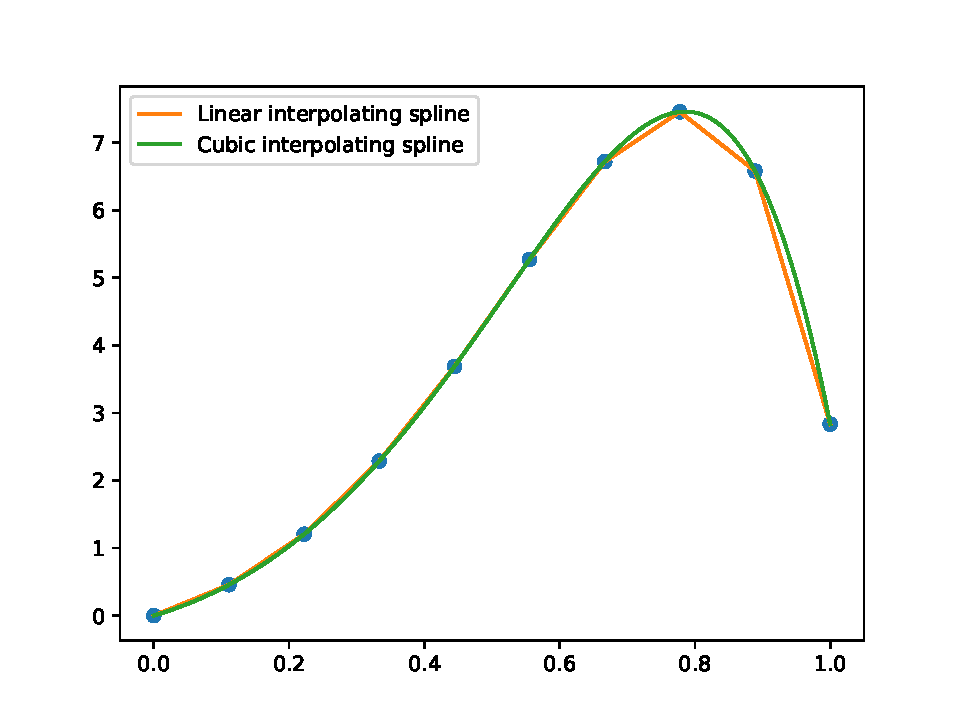
\includegraphics[width=0.60\textwidth]{spline}

  \begin{itemize}
  \item Defined piecewsise by polinomials of degree k ($k = 3$ fairly popular)
    \begin{itemize}
    \item Interpolating: passing through a set of pre-defined points
    \item First $k-1$ derivatives continuos at the control points
    \end{itemize}
  \item Superior to polynomial interpolation or curve fitting in many cases
  \end{itemize}
\end{frame}


\begin{frame}
  \frametitle{Splines: construction and properties}
  \begin{Verbatim}[label=\makebox{\url{https://github.com/lucabaldini/cmepda/tree/master/slides/latex/snippets/spline.py}},commandchars=\\\{\}]
\PY{k+kn}{import} \PY{n+nn}{numpy} \PY{k+kn}{as} \PY{n+nn}{np}
\PY{k+kn}{from} \PY{n+nn}{scipy.interpolate} \PY{k+kn}{import} \PY{n}{InterpolatedUnivariateSpline}

\PY{n}{x} \PY{o}{=} \PY{n}{np}\PY{o}{.}\PY{n}{linspace}\PY{p}{(}\PY{l+m+mf}{0.}\PY{p}{,} \PY{l+m+mf}{1.}\PY{p}{,} \PY{l+m+mi}{10}\PY{p}{)}
\PY{n}{y} \PY{o}{=} \PY{n}{np}\PY{o}{.}\PY{n}{exp}\PY{p}{(}\PY{l+m+mf}{3.} \PY{o}{*} \PY{n}{x}\PY{p}{)} \PY{o}{*} \PY{n}{np}\PY{o}{.}\PY{n}{sin}\PY{p}{(}\PY{l+m+mf}{3.} \PY{o}{*} \PY{n}{x}\PY{p}{)}

\PY{n}{s1} \PY{o}{=} \PY{n}{InterpolatedUnivariateSpline}\PY{p}{(}\PY{n}{x}\PY{p}{,} \PY{n}{y}\PY{p}{,} \PY{n}{k}\PY{o}{=}\PY{l+m+mi}{1}\PY{p}{)}
\PY{n}{s3} \PY{o}{=} \PY{n}{InterpolatedUnivariateSpline}\PY{p}{(}\PY{n}{x}\PY{p}{,} \PY{n}{y}\PY{p}{,} \PY{n}{k}\PY{o}{=}\PY{l+m+mi}{3}\PY{p}{)}

\PY{k}{print}\PY{p}{(}\PY{n}{s1}\PY{p}{(}\PY{l+m+mf}{0.234}\PY{p}{)}\PY{p}{)}
\PY{k}{print}\PY{p}{(}\PY{n}{s1}\PY{o}{.}\PY{n}{integral}\PY{p}{(}\PY{l+m+mf}{0.2}\PY{p}{,} \PY{l+m+mf}{0.8}\PY{p}{)}\PY{p}{)}

[Output]
1.3192110648078448
2.6659857771053925
\end{Verbatim}
  
  \begin{itemize}
  \item Evaluation is fairly inexpensive
    \begin{itemize}
    \item If the input $x$-array is sorted can do a binary search in
      \alert{O(log(N)) complexity}
    \end{itemize}
  \item Derivatives and integrals are easy
    \begin{itemize}
    \item Can be calculated \emph{exactly} by means of elementary
      arithmetic operations
    \end{itemize}
  \end{itemize}
\end{frame}


\begin{frame}
  \frametitle{References}
  \scriptsize
  \begin{itemize}
  \item \url{https://numpy.org/}
  \item \url{https://www.scipy.org/}
  \item \url{https://docs.scipy.org/doc/numpy/reference/arrays.indexing.html}
  \item \url{https://docs.scipy.org/doc/numpy/user/basics.broadcasting.html}
  \item \url{https://docs.scipy.org/doc/scipy/reference/interpolate.html}
  \end{itemize}
\end{frame}



\end{document}
